% Brimstone Maximizer - manuel d'utilisation.
% pdflatex manuel.tex (trois passes) ; figures : python3 figures.py (doc/fig_*.pdf).
% Copyright (C) 2026 Brimstone authors - SPDX-License-Identifier: GPL-2.0-or-later
\documentclass[a4paper,11pt]{article}
\usepackage[T1]{fontenc}
\usepackage[utf8]{inputenc}
\usepackage[french]{babel}
\usepackage{lmodern}
\usepackage{microtype}
\usepackage[margin=2.3cm]{geometry}
\usepackage{amsmath,amssymb}
\usepackage{graphicx}
\usepackage{booktabs}
\usepackage{array}
\usepackage{tabularx}
\usepackage{xcolor}
\usepackage{tikz}
\usetikzlibrary{arrows.meta,positioning,fit,calc}
\usepackage{enumitem}
\usepackage[hidelinks]{hyperref}

\definecolor{ember}{HTML}{C2410C}
\definecolor{ochre}{HTML}{A8650F}
\definecolor{ink}{HTML}{2A2421}
\definecolor{paper}{HTML}{F6F2EC}

\newcommand{\ctl}[1]{\textsf{\textbf{#1}}}   % nom d'un élément de l'interface
\newcommand{\dB}{\,dB}
\newcommand{\dBFS}{\,dBFS}
\setlist{itemsep=1pt,topsep=3pt}
\emergencystretch=3em
\graphicspath{{./}{../}}

\title{\textcolor{ember}{\textbf{BRIMSTONE}} \textsf{MAXIMIZER}\\[4pt]
\large Manuel d'utilisation et description de l'algorithme}
\author{Version 1.1.0}
\date{}

\begin{document}
\maketitle

\begin{center}
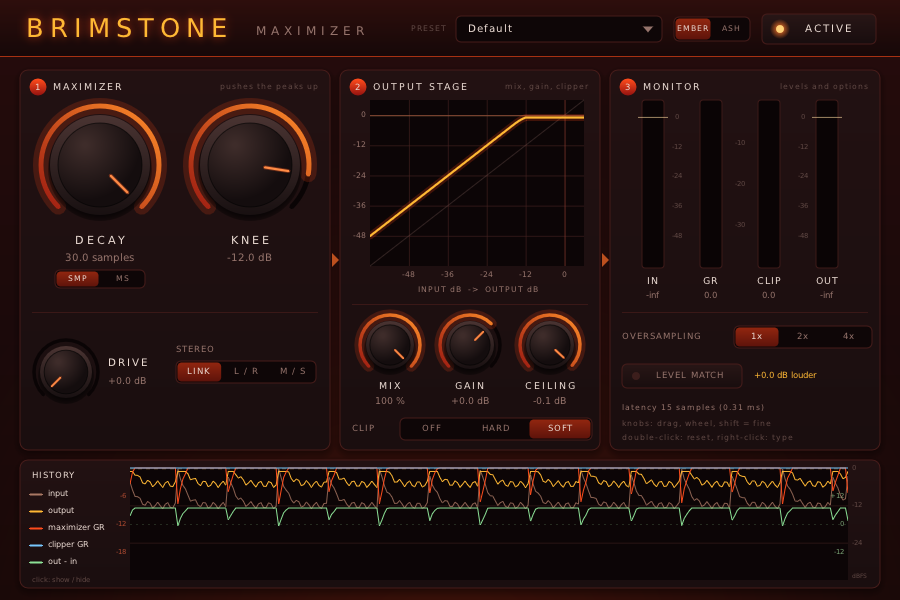
\includegraphics[width=0.92\textwidth]{capture_interface.png}
\end{center}

\newpage
\tableofcontents
\newpage

% ==============================================================================================
\section{Présentation}

Brimstone Maximizer est un maximiseur de crêtes : il rend un signal plus fort en ramenant
chaque crête qui dépasse un seuil (le \emph{knee}) au niveau du plafond de sortie, et en
amplifiant d'autant tout ce qui reste sous ce seuil. Son cœur reprend exactement l'algorithme du
\og Barry's Satan Maximiser\fg{} (greffon LADSPA \texttt{satan\_maximiser} des swh-plugins de
Steve Harris) ; autour de ce cœur, Brimstone ajoute ce qui manque pour un usage en mastering ou
en mixage : plafond de sortie, écrêteur doux ou dur, suréchantillonnage, mélange avec le signal
sec, modes stéréo, écoute de la différence, comparaison à sonie égale, préréglages.

Le son du cœur est volontairement brutal : la réduction de gain est instantanée et l'anticipation
courte. Selon les réglages, Brimstone va du limiteur discret (Knee faible, Mix partiel, écrêteur
doux) à la distorsion franche (Decay court, Knee très bas).

\paragraph{Formats.} VST3 et CLAP pour Windows 64 bits ; VST3, CLAP et LV2 pour Linux. Le greffon
est stéréo (deux entrées, deux sorties) et déclare sa latence à l'hôte.

\paragraph{Licence.} GPL 2 ou ultérieure, comme l'original (fichier \texttt{COPYING}). L'interface
et l'adaptation aux formats reposent sur DPF (licence ISC).

% ==============================================================================================
\section{Installation}

\paragraph{Windows.} Lancer \texttt{Brimstone-Maximizer-1.1.0-setup.exe} : il installe le VST3
(obligatoire) et, si on le coche, le CLAP, puis ajoute un désinstalleur (\og Programmes et
fonctionnalités\fg). À la main : copier le dossier \texttt{brimstone\_maximizer.vst3} dans
\verb|C:\Program Files\Common Files\VST3\| et \texttt{brimstone\_maximizer.clap} dans
\verb|C:\Program Files\Common Files\CLAP\|.

\paragraph{Linux.} Copier \texttt{brimstone\_maximizer.vst3} dans \verb|~/.vst3/|,
\texttt{brimstone\_maximizer.clap} dans \verb|~/.clap/| ou \texttt{brimstone\_maximizer.lv2}
dans \verb|~/.lv2/|.

Relancer ensuite l'analyse des greffons de l'hôte. Le désinstalleur laisse les préférences et
les préréglages de l'utilisateur (section~\ref{sec:fichiers}).

% ==============================================================================================
\section{Prise en main en une minute}

\begin{enumerate}
\item Insérer Brimstone en dernier sur la piste ou le bus de mixage. Le préréglage
  \ctl{Default} est chargé : Knee $-12$\dB, plafond $-0{,}1$\dBFS, écrêteur doux.
\item Baisser \ctl{KNEE} pour gagner en niveau (chaque dB de Knee en moins est un dB de plus sur
  tout ce qui est sous le seuil) ; écouter quand le son commence à se tasser.
\item Régler \ctl{DECAY} : court, le son est plus dur et plus granuleux ; long, plus lisse.
\item Activer \ctl{LEVEL MATCH} et basculer \ctl{BYPASS} : on compare à sonie égale, sans
  être trompé par le gain de niveau. \ctl{DELTA} fait entendre ce que le traitement retire.
\end{enumerate}

% ==============================================================================================
\section{L'interface}

La fenêtre (900 × 600 points, redimensionnable en gardant ses proportions) se lit de gauche à
droite dans l'ordre du signal : trois sections numérotées reliées par des flèches, puis
l'historique en bas. Chaque élément a une bulle d'aide au survol.

\subsection{En-tête}
\begin{description}
\item[Préréglages.] Liste déroulante : un clic l'ouvre ; elle montre les préréglages d'usine
  (\ctl{FACTORY}), un trait, vos préréglages (\ctl{USER}, par ordre alphabétique), un trait, puis
  \ctl{Save current settings\ldots}. Le préréglage courant est marqué d'un point ; \og *\fg{}
  après son nom signale un réglage modifié depuis son chargement. La molette sur la boîte fermée
  passe au préréglage suivant ou précédent. Détails en section~\ref{sec:prereglages}.
\item[A | B et A>B.] Deux jeux de réglages à comparer : un clic sur \ctl{A} ou \ctl{B} bascule
  (le jeu quitté est gardé, l'autre est rechargé ; à la première visite, B part d'une copie de
  A). \ctl{A>B} (ou \ctl{B>A}) copie le jeu courant dans l'autre. Les deux jeux sont
  enregistrés avec le projet. Avec Level match, on compare deux réglages à sonie égale.
\item[EMBER | ASH.] Thème sombre ou clair, sans effet sur le son ; c'est une préférence de
  l'ordinateur, commune à toutes les instances et à tous les projets.
\item[ACTIVE / BYPASSED.] Le Bypass déclaré à l'hôte (section~\ref{sec:bypass}).
\end{description}

\subsection{Section 1 : MAXIMIZER}
\ctl{DECAY} (et son unité \ctl{SMP | MS}), \ctl{KNEE}, \ctl{DRIVE}, \ctl{STEREO}. La section
est grisée, avec la mention \og OFF: mix at 0 \%\fg, quand Mix est à 0\,\% : le maximiseur
est alors hors circuit et Brimstone n'est plus qu'un écrêteur.

\subsection{Section 2 : OUTPUT STAGE}
La courbe de transfert donne le niveau de sortie pour un niveau d'entrée stable, tous réglages
compris ; un point suit le niveau d'entrée courant. Dessous : \ctl{MIX}, \ctl{GAIN},
\ctl{CEILING}, le sélecteur \ctl{CLIP} (\ctl{OFF | HARD | SOFT}) et le petit bouton
\ctl{SOFT KNEE} à sa droite (grisé hors Soft).

\subsection{Section 3 : MONITOR}
Vu-mètres \ctl{IN} (crête d'entrée), \ctl{GR} (réduction du maximiseur), \ctl{CLIP} (réduction
de l'écrêteur), \ctl{OUT} (crête de sortie) ; \ctl{OVERSAMPLING} (1x, 2x, 4x) ; \ctl{LEVEL
MATCH} et \ctl{DELTA} ; l'écart de sonie entre sortie et entrée en LU ; la latence.

\subsection{Historique}
Cinq courbes fines sur une même bande, un point toutes les 25\,ms : \emph{input} et
\emph{output} (crêtes, montent depuis le bas, dBFS, échelle de droite ; pointillés : plafond),
\emph{maximizer GR} et \emph{clipper GR} (réductions, descendent depuis le haut, échelle de
gauche), \emph{out - in} (gain total réellement appliqué, échelle centrée sur 0 graduée dans le
graphique). Chaque point est la crête des 30 dernières millisecondes : aucune crête n'est perdue
entre deux points. Un clic sur une légende montre ou cache sa courbe ; le sélecteur \ctl{3 s |
7 s | 30 s} règle la durée affichée. Ces deux choix sont enregistrés avec le projet.

\subsection{Manipuler les boutons}
\begin{itemize}
\item glisser verticalement ; \textsf{Maj} pour un réglage fin ;
\item molette (\textsf{Maj} : fin) ;
\item double-clic ou \textsf{Ctrl}+clic : valeur par défaut ;
\item clic droit : saisie de la valeur au clavier (\textsf{Entrée} valide, \textsf{Échap}
  annule ; la virgule est acceptée comme séparateur décimal).
\end{itemize}

% ==============================================================================================
\section{Les réglages}

\begin{center}
\small
\begin{tabularx}{\textwidth}{@{}l l l X@{}}
\toprule
Réglage & Plage & Défaut & Rôle \\
\midrule
Decay & 2--30 éch. ou 0,05--2\,ms & 30 éch. & retour de l'enveloppe et anticipation ; bouton SMP/MS \\
Knee & $-90$--0\dB & $-12$\dB & seuil : au-dessus, les crêtes sont ramenées au plafond \\
Drive & 0--24\dB & 0\dB & gain d'entrée du seul signal traité \\
Stereo & Link, L/R, M/S & Link & détection commune, par canal ou milieu/côtés \\
Mix & 0--100\,\% & 100\,\% & part du signal traité ; 0\,\% : maximiseur hors circuit \\
Gain & $-24$--+12\dB & 0\dB & après le mélange, avant l'écrêteur \\
Ceiling & $-12$--0\dB & $-0{,}1$\dB & niveau de sortie maximal \\
Clip & Off, Hard, Soft & Soft & écrêtage au plafond \\
Soft knee & 0,1--6\dB & 1\dB & en Soft, début de l'arrondi sous le plafond \\
Oversampling & 1x, 2x, 4x & 1x & fréquence interne du traitement \\
Level match & oui/non & non & compense le gain de sonie \\
Delta & oui/non & non & fait entendre la différence \\
Bypass & oui/non & non & entrée retardée de la latence \\
\bottomrule
\end{tabularx}
\end{center}

\paragraph{Decay.} Règle à la fois la vitesse à laquelle le gain remonte après une crête et
l'anticipation (la moitié du Decay). Dans l'unité d'origine (\ctl{SMP}), il est compté en
échantillons à la fréquence de l'hôte, quel que soit le suréchantillonnage : 30 échantillons
font 0,68\,ms à 44,1\,kHz mais 0,31\,ms à 96\,kHz. En \ctl{MS}, le son est le même à toute
fréquence. La bascule convertit la valeur pour garder la même constante de temps.

\paragraph{Knee.} C'est le niveau au-dessus duquel une crête est \og aplatie\fg{} au plafond.
Tout ce qui est sous le Knee est amplifié de $-\mathrm{Knee}$ (+12\dB{} pour $-12$\dB), puis
placé sous le plafond. Baisser le Knee augmente donc le niveau moyen d'autant, et la réduction de
gain sur les crêtes.

\paragraph{Drive.} Amplifie l'entrée du maximiseur seulement : le signal sec du mélange n'est pas
changé. Avec un Mix partiel, Drive pousse le maximiseur plus fort sans changer la part du sec.

\paragraph{Stereo.} \ctl{LINK} : un seul détecteur pour les deux canaux (le plus fort des deux),
l'image stéréo est préservée. \ctl{L / R} : chaque canal a son détecteur, comme l'original ;
l'image peut bouger quand un seul canal crête. \ctl{M / S} : le traitement porte sur le milieu
$(L+R)/2$ et les côtés $(L-R)/2$, chacun avec son détecteur.

\paragraph{Mix, Gain, Ceiling.} Le signal traité (mis au plafond) est mélangé au signal sec,
puis \ctl{GAIN} pousse le tout vers l'écrêteur. \ctl{CEILING} est le niveau maximal de sortie
quand l'écrêteur est actif.

\paragraph{Clip et Soft knee.} \ctl{OFF} : comme l'original, la sortie n'est pas bornée ; elle
peut dépasser le plafond de plusieurs dB (section~\ref{sec:depassement}). \ctl{HARD} : tout ce
qui dépasse est coupé net au plafond. \ctl{SOFT} : le signal est linéaire jusqu'au Soft knee
(sous le plafond), puis arrondi jusqu'au plafond sans jamais l'atteindre brutalement.

\paragraph{Oversampling.} Fait tourner tout le traitement à 2 ou 4 fois la fréquence de l'hôte :
moins de repliement (aliasing) des distorsions, plus de latence et de calcul.

\paragraph{Level match, Delta, Bypass.} Voir sections~\ref{sec:mesures} et~\ref{sec:bypass}.

% ==============================================================================================
\section{Préréglages}\label{sec:prereglages}

\subsection{Préréglages d'usine}
\begin{center}
\small
\begin{tabular}{@{}l r r r r r l l r r l r@{}}
\toprule
Nom & Decay & Knee & Drive & Ceil. & Clip & S.\,knee & Stereo & Mix & Gain & OS \\
\midrule
Default        & 30 éch.  & $-12$ & 0  & $-0{,}1$ & Soft & 1    & Link & 100 & 0    & 1x \\
Original (swh) & 30 éch.  & $-12$ & 0  & 0        & Off  & --   & L/R  & 100 & 0    & 1x \\
Subtle         & 30 éch.  & $-6$  & 0  & $-0{,}3$ & Soft & 2    & Link & 60  & 0    & 2x \\
Loud master    & 1,5\,ms  & $-14$ & 3  & $-0{,}3$ & Soft & 1    & Link & 100 & 0    & 4x \\
Wide crush     & 12 éch.  & $-24$ & 0  & $-0{,}5$ & Soft & 4,44 & M/S  & 70  & 0    & 2x \\
Destruction    & 2 éch.   & $-45$ & 12 & $-1$     & Hard & --   & L/R  & 100 & $-3$ & 1x \\
Clipper        & 30 éch.  & $-12$ & 0  & $-0{,}3$ & Hard & --   & L/R  & 0   & +3   & 4x \\
\bottomrule
\end{tabular}
\end{center}
Niveaux en dB, Mix en \%. \og Original (swh)\fg{} reproduit l'original à l'échantillon près
(retardé de 15 échantillons). \og Clipper\fg{} met le maximiseur hors circuit (Mix 0\,\%) : le
signal passe seulement par Gain (+3\dB) et l'écrêtage dur à $-0{,}3$\dB, en 4x. Les préréglages
d'usine sont aussi présentés à l'hôte (liste des programmes).

\subsection{Vos préréglages}
\begin{description}
\item[Enregistrer.] Dans la liste, \ctl{Save current settings\ldots}, puis taper le nom
  directement dans la boîte (proposé : le nom de votre préréglage en cours). \textsf{Entrée}
  enregistre, \textsf{Échap} ou un clic ailleurs annule. Une bulle dit ce que fera
  \textsf{Entrée} : enregistrer, remplacer votre préréglage du même nom (majuscules et minuscules
  confondues), ou refuser : nom d'un préréglage d'usine, nom invalide, dossier non inscriptible.
  Noms : 1 à 24 caractères ASCII imprimables, sans \verb|< > : " / \ | ? *|, sans espace ni point
  au début ou à la fin, ni nom réservé de Windows (\texttt{CON}, \texttt{NUL}\ldots).
\item[Supprimer.] Survoler votre préréglage dans la liste : une croix apparaît à droite. Un
  premier clic affiche \og delete?\fg, un second supprime (sans retour en arrière).
\item[Portée.] Vos préréglages sont communs à tous les projets, toutes les instances et tous les
  hôtes de l'ordinateur ; la liste est relue à chaque ouverture, le fichier à chaque chargement.
  L'hôte, lui, ne voit que les préréglages d'usine ; ses propres préréglages (par exemple
  \texttt{.vstpreset}) restent possibles et indépendants.
\end{description}
Bypass et Delta, qui servent à l'écoute, ne font partie d'aucun préréglage ni du jeu A/B.

% ==============================================================================================
\section{L'algorithme}

Cette section décrit exactement le calcul fait par le greffon (fichier
\nolinkurl{plugin/BrimstonePlugin.cpp}). Les courbes sont calculées avec les mêmes formules.

\subsection{Chaîne du signal}

\begin{center}
\begin{tikzpicture}[
  node distance=4mm and 4mm,
  blk/.style={draw=ink, rounded corners=2pt, fill=paper, minimum height=7mm, align=center,
              font=\footnotesize\sffamily, inner sep=3pt},
  core/.style={blk, fill=ember!15, draw=ember},
  arr/.style={-{Stealth[length=2mm]}, ink}]
\node[blk] (in) {entrée\\$x$};
\node[blk, right=of in] (up) {suréch.\\1x/2x/4x};
\node[blk, right=of up] (drv) {Drive};
\node[blk, right=of drv] (ms) {M/S\\(option)};
\node[core, right=of ms] (cor) {cœur :\\enveloppe, gain};
\node[blk, right=of cor] (ceil) {× plafond};
\node[blk, below=10mm of ceil] (mix) {mélange\\sec/traité};
\node[blk, left=of mix] (gain) {Gain};
\node[blk, left=of gain] (clip) {écrêteur\\Hard/Soft};
\node[blk, left=of clip] (down) {sous-éch.};
\node[blk, left=of down] (safe) {borne de\\sûreté};
\node[blk, left=of safe] (lm) {Level match\\ou Delta};
\node[blk, below=10mm of lm] (byp) {Bypass\\(fondu)};
\node[blk, right=of byp] (out) {sortie};
\draw[arr] (in) -- (up); \draw[arr] (up) -- (drv); \draw[arr] (drv) -- (ms);
\draw[arr] (ms) -- (cor); \draw[arr] (cor) -- (ceil); \draw[arr] (ceil) -- (mix);
\draw[arr] (mix) -- (gain); \draw[arr] (gain) -- (clip); \draw[arr] (clip) -- (down);
\draw[arr] (down) -- (safe); \draw[arr] (safe) -- (lm); \draw[arr] (lm) -- (byp);
\draw[arr] (byp) -- (out);
\draw[arr, dashed] (up.north) -- ++(0,5mm) -| node[pos=0.25, above, font=\scriptsize] {signal sec, retardé de $L_{\mathrm{fix}}$} ($(ceil.east)+(4mm,0)$) |- (mix.east);
\draw[arr, dashed] (in.west) -- ++(-6mm,0) |- node[pos=0.25, left, font=\scriptsize, align=right] {entrée\\retardée\\de la\\latence} (byp.west);
\end{tikzpicture}
\end{center}

Tout ce qui est entre le suréchantillonnage et le sous-échantillonnage tourne à la fréquence
interne $f_i = k\,f_s$ ($f_s$ : fréquence de l'hôte, $k = 1, 2$ ou $4$). On note $x[n]$ un
échantillon interne d'un canal.

\subsection{Le cœur du maximiseur}\label{sec:coeur}

\paragraph{Enveloppe.} Pour chaque échantillon, avec $a[n] = |s[n]|$ le module du signal
($s = $ entrée × Drive, éventuellement en milieu/côtés) et $d$ le Decay en échantillons internes :
\[
e[n] =
\begin{cases}
a[n] & \text{si } a[n] > e[n-1] \quad\text{(attaque instantanée)}\\[2pt]
e[n-1] + \dfrac{a[n] - e[n-1]}{d} & \text{sinon (retour exponentiel)}
\end{cases}
\]
Le retour est un filtre du premier ordre de constante de temps $d$ échantillons : après une
crête, l'enveloppe perd environ 63\,\% de son écart au signal en $d$ échantillons. En mode
\ctl{LINK}, l'enveloppe est commune et suit $\max(a_L, a_R)$ ; sinon chaque canal (ou le milieu
et les côtés) a la sienne. $d = \mathrm{Decay} \times k$ dans l'unité d'origine,
$d = \mathrm{Decay_{ms}} \times 10^{-3} \times f_i$ en millisecondes, et au moins 2.

\paragraph{Gain.} Avec $K = 10^{\mathrm{Knee}/20}$ :
\[
g[n] = \frac{1}{\max\bigl(e[n],\, K\bigr)} .
\]
Sous le Knee, $g = 1/K$ est constant : c'est le gain de compensation (\emph{makeup}), +12\dB{}
pour un Knee de $-12$\dB. Au-dessus, $g = 1/e$ : la crête est ramenée à 1, puis multipliée par
le plafond $C = 10^{\mathrm{Ceiling}/20}$. Le gain ne dépend que du module : le maximiseur ne
déforme pas la forme d'onde au-delà de la modulation de gain.

\paragraph{Anticipation.} Le gain appliqué à l'échantillon $x[n]$ est celui calculé
$a = \operatorname{round}(d/2)$ échantillons plus tard :
\[
y_{\text{traité}}[n] = s[n]\; g[n+a]\; C .
\]
Comme l'attaque de l'enveloppe est instantanée, la réduction commence donc $a$ échantillons
\emph{avant} la crête (le signal est retardé, la détection ne l'est pas), puis le gain remonte
au rythme du Decay (figure~\ref{fig:temps}). C'est exactement l'original, où le signal est
retardé de $a$ échantillons et le gain appliqué sans retard.

\begin{figure}[htbp]
\centering
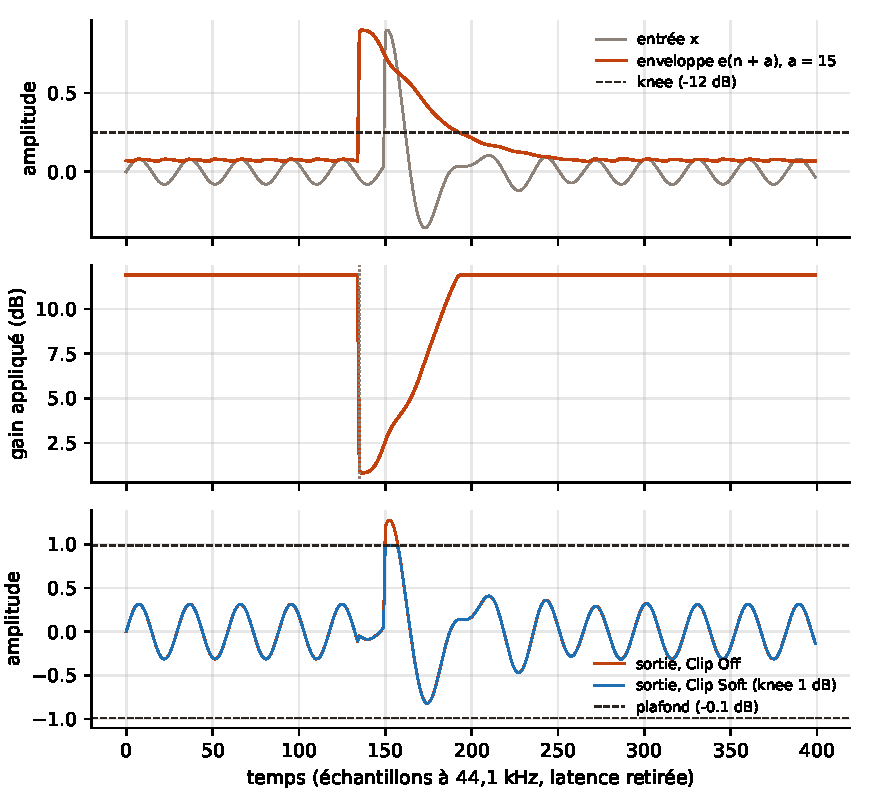
\includegraphics[width=0.82\textwidth]{fig_temps.pdf}
\caption{Une frappe sur un son faible, Decay 30 échantillons, Knee $-12$\dB{} (1x, 44,1\,kHz).
En haut : entrée et enveloppe vue au moment où le gain est appliqué ; au milieu : gain total
(compensation et plafond compris) ; en bas : sortie sans écrêteur, qui dépasse le plafond de
+2,2\dB{} sur la frappe, et avec l'écrêteur doux.}
\label{fig:temps}
\end{figure}

\paragraph{Courbe statique.} Pour un signal stable de niveau $x$, $e = x$ et la sortie vaut
$x \cdot C/\max(x,K)$ : linéaire avec un gain $C/K$ sous le Knee, plate au plafond au-dessus
(figure~\ref{fig:transfert}). Le Mix mélange cette courbe à la diagonale.

\begin{figure}[htbp]
\centering
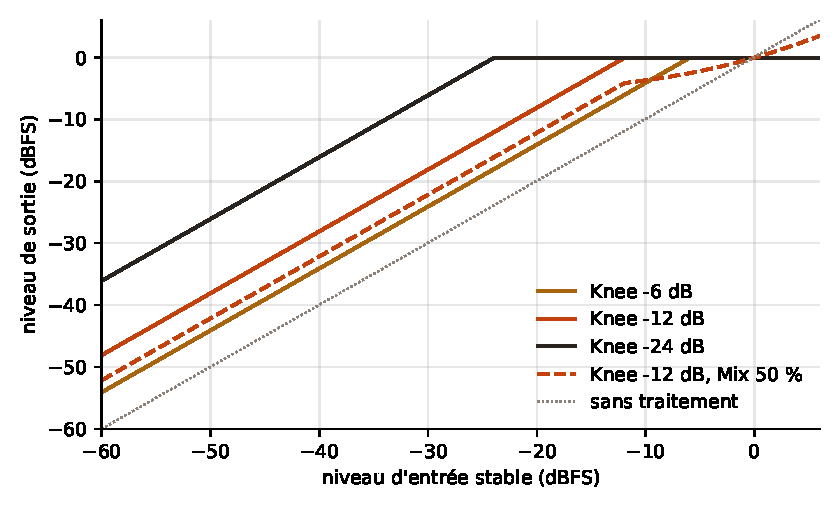
\includegraphics[width=0.66\textwidth]{fig_transfert.pdf}
\caption{Niveau de sortie pour un niveau d'entrée stable (Clip Off, plafond $-0{,}1$\dB).}
\label{fig:transfert}
\end{figure}

\paragraph{Dépassement du plafond.}\label{sec:depassement} Au moment où une crête isolée joue,
l'enveloppe a déjà décru pendant $a$ échantillons depuis qu'elle l'a captée : le gain est un peu
trop fort et la sortie dépasse le plafond. Au pire (crête isolée suivie de silence), le facteur
est $(1-1/d)^{-a}$ : +4,4\dB{} pour un Decay de 30 échantillons, +6,0\dB{} pour 2 et jusqu'à
+7,0\dB{} pour 3 (l'anticipation y est arrondie à 2 échantillons ; figure~\ref{fig:depassement}),
tant que l'enveloppe reste au-dessus du Knee ; sinon le gain est celui de compensation et le
dépassement vaut au plus $|x|/K$. Vérifié sur le greffon (Original, impulsion à 0\dBFS) :
+6,02, +7,04, +5,00 et +4,42\dB{} pour des Decay de 2, 3, 4 et 30. C'est le comportement de l'original, conservé en \ctl{Clip OFF} ;
les modes \ctl{HARD} et \ctl{SOFT} le corrigent.

\begin{figure}[htbp]
\centering
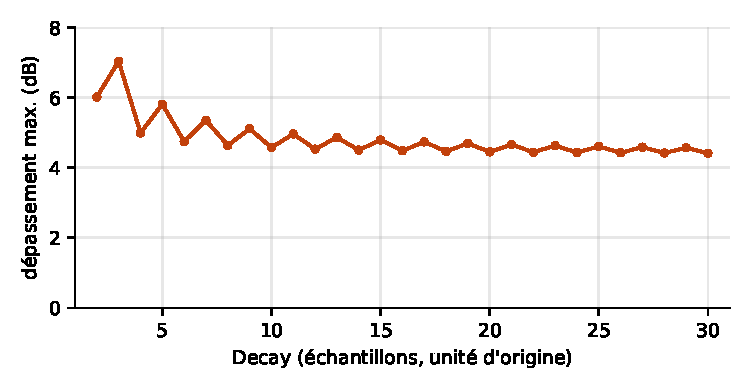
\includegraphics[width=0.6\textwidth]{fig_depassement.pdf}
\caption{Dépassement maximal du plafond sans écrêteur, selon le Decay.}
\label{fig:depassement}
\end{figure}

\paragraph{Changer le Decay sans clic.} L'anticipation $a$ dépend du Decay. Pour que la latence
ne change pas, le signal est toujours retardé d'un nombre fixe $L_{\mathrm{fix}}$ d'échantillons
(l'anticipation maximale) et le gain de $L_{\mathrm{fix}} - a$. Quand $a$ change, un second
détecteur (enveloppe et historique des gains) démarre depuis l'état du premier avec la nouvelle
anticipation, et les deux gains sont fondus linéairement en 5\,ms. Chaque détecteur reste
cohérent avec son anticipation : ni clic, ni dépassement pendant le changement.

\subsection{Mélange, gain et écrêteur}

Pour chaque canal :
\[
y[n] = \bigl(x_{\text{sec}}[n] + (y_{\text{traité}}[n] - x_{\text{sec}}[n])\,M\bigr)\, G ,
\]
avec $M$ le Mix (0 à 1), $G = 10^{\mathrm{Gain}/20}$ et $x_{\text{sec}}$ l'entrée (sans Drive)
retardée comme le signal traité. En M/S, le traité est repassé en gauche/droite avant le mélange.
À Mix 0\,\%, la sortie ne dépend plus du maximiseur : il ne reste que Gain et l'écrêteur.

\paragraph{Écrêteur.} Avec $C$ le plafond et, en Soft, $t = C\cdot 10^{-\mathrm{Soft\,knee}/20}$
le début de l'arrondi :
\[
\text{Hard : } y_c = \max(-C, \min(y, C)), \qquad
\text{Soft : } |y_c| =
\begin{cases}
|y| & \text{si } |y| \le t\\
t + (C - t)\tanh\dfrac{|y| - t}{C - t} & \text{sinon}
\end{cases}
\]
La courbe Soft est continue et de pente continue en $t$ (pente 1), et tend vers $C$ sans
l'atteindre (figure~\ref{fig:ecreteur}). Une crête poussée exactement au plafond par le
maximiseur ressort à $t + (C-t)\tanh 1$ : $-0{,}23$\dB{} sous le plafond pour un Soft knee de
1\dB, $-0{,}45$\dB{} pour 2\dB, $-0{,}87$\dB{} pour 4,44\dB{} (60\,\% du plafond, le
réglage de Wide crush). Un petit Soft knee rapproche du Hard et garde le niveau ; un grand arrondit
davantage et sonne plus doux.

\begin{figure}[htbp]
\centering
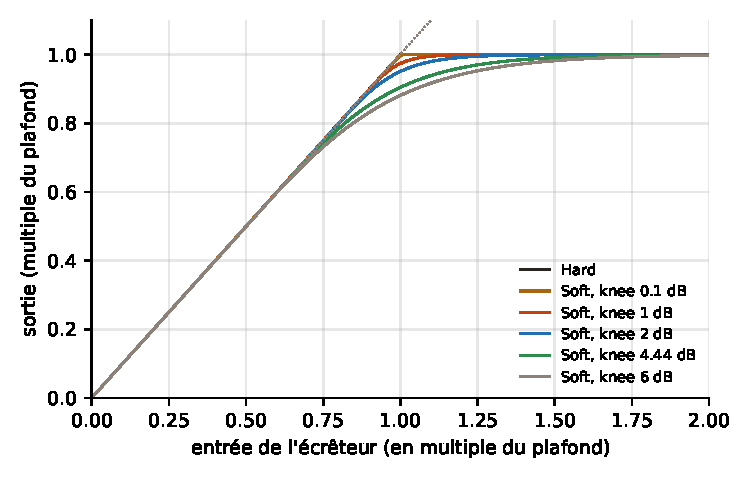
\includegraphics[width=0.6\textwidth]{fig_ecreteur.pdf}
\caption{Écrêteur Hard et Soft selon le Soft knee (amplitudes en multiples du plafond).}
\label{fig:ecreteur}
\end{figure}

\paragraph{Borne de sûreté.} Le filtre de sous-échantillonnage peut faire osciller légèrement le
signal au-dessus du plafond ; quand Clip est Hard ou Soft, la sortie est donc bornée une seconde
fois au plafond, à la fréquence de l'hôte. Le plafond est garanti sur les échantillons ; les
crêtes \emph{entre} les échantillons (après conversion analogique) peuvent le dépasser
légèrement : laisser quelques dixièmes de dB de marge pour un fichier destiné à un codage avec
perte.

\subsection{Suréchantillonnage}

Les étages 2x sont des filtres demi-bande à phase linéaire (sinus cardinal fenêtré par Kaiser,
$\beta = 8$), en forme polyphasée : montée (insertion d'un zéro sur deux puis filtrage) et
descente (filtrage puis un échantillon sur deux). L'étage qui coupe à la fréquence de Nyquist de
l'hôte a 107 coefficients ; le 4x lui ajoute un second étage de 47 coefficients, qui coupe à la
fréquence de l'hôte (bien au-dessus de l'audible). Le retard d'un aller-retour est de 106
échantillons à 2 fois la fréquence de l'hôte pour le premier étage, 46 à 4 fois pour le second.

\begin{figure}[htbp]
\centering
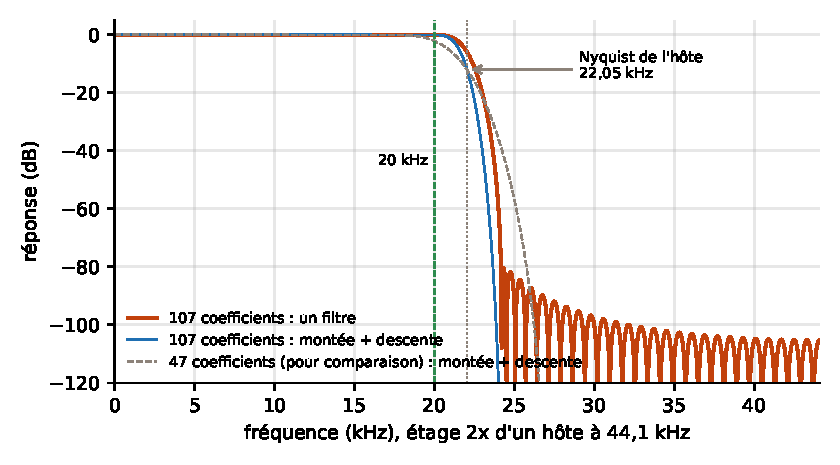
\includegraphics[width=0.7\textwidth]{fig_demi_bande.pdf}
\caption{Réponse de l'étage 2x pour un hôte à 44,1\,kHz.}
\label{fig:demibande}
\end{figure}

Pour un hôte à 44,1\,kHz, la bande de transition va de 20,1 à 24,2\,kHz : la réponse est plate
à 0,01\dB{} près jusqu'à 20\,kHz et la réjection dépasse 80\dB{} au-delà de 24,2\,kHz, si bien
que ce que la distorsion crée au-dessus de la fréquence de Nyquist ne revient pas en repliement
dans l'audible. Mesuré sur le greffon (Mix 0, Clip Off, montée et descente) : $-0{,}006$\dB{} à
20\,kHz, $-1{,}3$\dB{} à 21\,kHz. À 48\,kHz, ces fréquences montent d'environ 9\,\%.

Pour comparaison, un filtre de 47 coefficients (courbe en tirets, celui du second étage)
laisserait une transition de 17,6 à 27\,kHz : aigu atténué de 2,0\dB{} à 20\,kHz et rejet de
19\dB{} seulement à 24,1\,kHz. Les 107 coefficients coûtent 30 échantillons de latence (0,7\,ms
à 44,1\,kHz) et environ 45\,\% de calcul en plus en 2x, 25\,\% en 4x.

\subsection{Latence}

La latence ne dépend que de l'unité du Decay et du suréchantillonnage ; elle est déclarée à
l'hôte, qui la compense. Avec $L_{\max}$ l'anticipation maximale en échantillons internes
($\operatorname{round}(30k/2)$ dans l'unité d'origine, $\operatorname{round}(2\,\mathrm{ms}\cdot
f_i/2)$ en millisecondes) et $S$ le retard des filtres (0, 106 ou 258 échantillons internes en
1x, 2x, 4x), le signal est retardé de $L_{\mathrm{fix}} = L_{\max} + p$ (le plus petit $p \ge 0$
qui rend $S + L_{\mathrm{fix}}$ multiple de $k$) et la latence vaut $(S + L_{\mathrm{fix}})/k$
échantillons de l'hôte.

\begin{center}
\small
\begin{tabular}{@{}l c c c c c c@{}}
\toprule
 & \multicolumn{3}{c}{Decay en échantillons} & \multicolumn{3}{c}{Decay en ms} \\
\cmidrule(lr){2-4}\cmidrule(lr){5-7}
Hôte & 1x & 2x & 4x & 1x & 2x & 4x \\
\midrule
44,1\,kHz & 15 (0,34\,ms) & 68 (1,54) & 80 (1,81) & 44 (1,00) & 97 (2,20) & 109 (2,47) \\
48\,kHz   & 15 (0,31) & 68 (1,42) & 80 (1,67) & 48 (1,00) & 101 (2,10) & 113 (2,35) \\
96\,kHz   & 15 (0,16) & 68 (0,71) & 80 (0,83) & 96 (1,00) & 149 (1,55) & 161 (1,68) \\
\bottomrule
\end{tabular}
\end{center}
Changer l'unité du Decay ou le suréchantillonnage change la latence et remet l'état du
traitement à zéro (court silence) ; les autres réglages se changent en cours de lecture.

\subsection{Lissage des réglages}

Knee, Drive, Ceiling, Mix, Gain et Soft knee sont lissés par un filtre du premier ordre de
10\,ms à la fréquence interne : tourner un bouton pendant la lecture ne produit pas de
crépitement. Bypass et Delta sont fondus en 10\,ms ; le changement de Decay est fondu en 5\,ms
(section~\ref{sec:coeur}).

\subsection{Bypass et Delta}\label{sec:bypass}

\paragraph{Bypass.} La sortie devient l'entrée retardée de la latence, exactement : pas de
décalage dans le temps à la bascule, et un fondu de 10\,ms évite le clic. Le traitement continue
pendant le Bypass, pour reprendre sans transitoire.

\paragraph{Delta.} Fait entendre ce que le maximiseur et l'écrêteur \emph{changent}, sans le
gain de compensation. La sortie est comparée à la même chaîne rendue linéaire : gain du
maximiseur tenu à sa valeur de compensation $1/K$ et pas d'écrêtage, soit
\[
y_{\text{lin}}[n] = x_{\text{sec}}[n]\,\Bigl(1 + \bigl(\tfrac{D\,C}{K} - 1\bigr) M\Bigr)\, G ,
\qquad \Delta[n] = y[n] - y_{\text{lin}}[n] ,
\]
($D$ : Drive linéaire), calculé à la fréquence interne puis sous-échantillonné par son propre
filtre, si bien que les filtres se compensent exactement. Sur une partie calme (sous le Knee),
Delta est nul ; sur une crête, on entend la réduction ; avec le préréglage Clipper, on entend
exactement ce que l'écrêteur coupe (figure~\ref{fig:delta}). Delta ignore Level match ; Bypass
est prioritaire.

\begin{figure}[htbp]
\centering
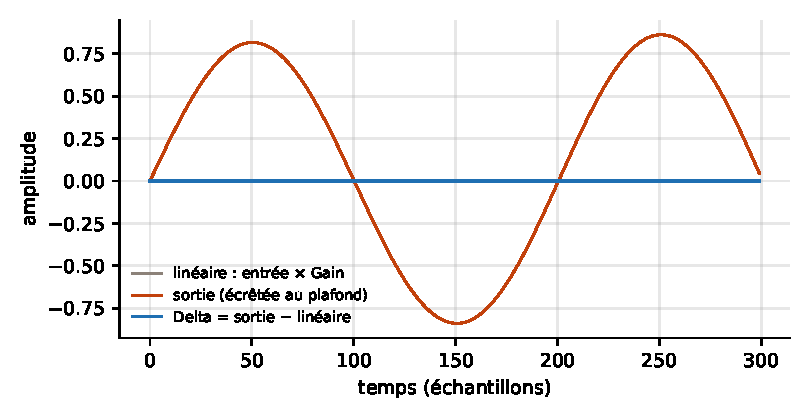
\includegraphics[width=0.68\textwidth]{fig_delta.pdf}
\caption{Delta avec le préréglage Clipper : la partie coupée par l'écrêteur.}
\label{fig:delta}
\end{figure}

\subsection{Mesures et écoute à sonie égale}\label{sec:mesures}

\paragraph{Vu-mètres.} \ctl{IN} et \ctl{OUT} : crêtes d'entrée et de sortie (dBFS), retour de
100\,ms. \ctl{GR} : réduction du maximiseur sous son gain de compensation, $g\,K$ en dB (0 quand
Mix est à 0\,\%). \ctl{CLIP} : réduction de l'écrêteur, $y_c/y$ en dB, borne de sûreté comprise.

\paragraph{Historique.} Le greffon garde, par tranches de 5\,ms, les crêtes d'entrée et de sortie
et les réductions maximales ; l'interface lit toutes les 25\,ms la crête des sept dernières
tranches (environ 30\,ms) : aucune crête n'échappe à l'affichage. \emph{out - in} est
$20\log_{10}(\text{sortie}/\text{entrée})$ sur ces crêtes, interrompu quand l'entrée est muette.

\paragraph{Sonie.} La sonie suit la recommandation ITU-R BS.1770 : chaque canal de l'entrée et de
la sortie passe par la pondération K (un plateau de +4\dB{} au-dessus d'environ 1,7\,kHz, puis
un passe-haut \og RLB\fg{} vers 38\,Hz, figure~\ref{fig:k}), puis on fait la moyenne
quadratique de la somme des canaux sur environ 1,5\,s (moyenne exponentielle, sans le
fenêtrage de la mesure intégrée). L'écart affiché est
\[
\Delta L = 10 \log_{10} \frac{\overline{y_K^2}}{\overline{x_K^2}} \quad \text{(LU, borné à } \pm 24\text{)} .
\]
Les coefficients sont calculés pour toute fréquence d'échantillonnage et valent ceux de la
norme à 48\,kHz. La pondération rend la comparaison plus proche de l'oreille qu'une moyenne
quadratique large bande, qui surestime les graves.

\begin{figure}[htbp]
\centering
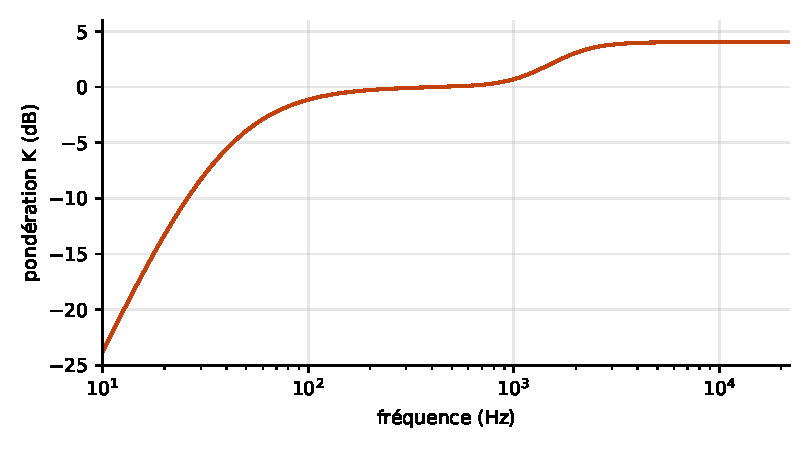
\includegraphics[width=0.66\textwidth]{fig_ponderation_k.pdf}
\caption{Pondération K de BS.1770 : $-3{,}9$\dB{} à 50\,Hz, +0,7\dB{} à 1\,kHz, +4,0\dB{} à
10\,kHz.}
\label{fig:k}
\end{figure}

\paragraph{Level match.} La sortie est multipliée par $10^{-\Delta L/20}$, rampe linéaire d'un
bloc audio au suivant : le traitement et le Bypass s'écoutent à sonie égale, ce qui évite de
préférer un réglage seulement parce qu'il est plus fort. La compensation suit la sonie avec
environ 1,5\,s de retard.

\subsection{Nombres dénormaux}

Dans un silence, l'enveloppe décroît vers zéro et finit sur le plus petit nombre dénormal
($1{,}4\times10^{-45}$), qu'elle ne quitte plus : multiplié par $1 - 1/d$, il s'arrondit à
lui-même. Sur x86, les calculs sur ces nombres sont très lents quand l'hôte laisse coupés les
modes FTZ/DAZ du processeur. Le greffon les active le temps de son calcul et rétablit l'état de
l'hôte en sortie : le coût d'un silence reste celui d'un signal ordinaire (deux à trois fois
moins qu'avant cette mesure, sur le banc \texttt{tests/bench\_cpu.cpp}). La sortie n'en est
changée qu'en dessous de $-400$\dBFS.

\subsection{Coût de calcul}
Mesuré sur un Intel i7-8665U (préréglage Default, stéréo, 44,1\,kHz, machine peu chargée ;
banc \texttt{tests/bench\_cpu.cpp}) : environ 47\,ns par trame stéréo en 1x, 165\,ns en 2x et
280\,ns en 4x, soit 0,2\,\%, 0,7\,\% et 1,2\,\% d'un cœur par instance. Delta ajoute un filtre de
sous-échantillonnage pendant qu'il est actif.

% ==============================================================================================
\section{Conseils d'utilisation}

\begin{description}
\item[Gagner du niveau sans se trahir.] Default, Knee entre $-6$ et $-10$\dB, Level match
  activé, et comparer avec Bypass. Si \ctl{GR} bat en permanence de plus de 6\dB, le son se
  tasse ; remonter le Knee ou baisser le Mix.
\item[Garder les transitoires.] Mix entre 50 et 80\,\% (compression parallèle) : le signal sec
  garde l'attaque, le maximiseur remplit le corps.
\item[Grave qui pompe.] Allonger le Decay (en ms : 1 à 2\,ms), ou passer en \ctl{M / S} pour que
  les côtés ne fassent pas pomper le milieu.
\item[Distorsion volontaire.] Decay 2 à 5 échantillons, Knee très bas, Drive : c'est le
  \og Satan\fg{} d'origine ; Clip Hard pour borner la sortie.
\item[Écrêteur seul.] Préréglage Clipper : Gain règle de combien on pousse ; 4x pour limiter le
  repliement. Delta fait entendre ce qui est coupé.
\item[Mastering.] 1x suffit souvent pour un maximiseur doux ; 2x ou 4x quand l'écrêteur
  travaille beaucoup (moins de repliement), au prix de 1,2 à 2,5\,ms de latence. Plafond à $-0{,}3$\dB{} ou plus bas
  pour un codage avec perte.
\item[Comparer deux réglages.] Régler A, copier vers B (\ctl{A>B}), modifier B, puis basculer A
  | B avec Level match actif.
\end{description}

% ==============================================================================================
\section{Fichiers, projets et compatibilité}\label{sec:fichiers}

\begin{description}
\item[Avec le projet.] Tous les réglages, le jeu A/B inactif, la durée de l'historique et les
  courbes affichées (états \texttt{ab} et \texttt{history}). Les réglages sont relus par leur
  nom : ajouter un réglage dans une version future ne casse pas un projet.
\item[Sur l'ordinateur.] Le thème dans \texttt{brimstone.conf} et vos préréglages dans
  \texttt{presets/}, un fichier \texttt{<nom>.preset} chacun, dans le dossier :
  \begin{itemize}
  \item Windows : \verb|%APPDATA%\Brimstone\| ;
  \item Linux : \verb|$XDG_CONFIG_HOME/brimstone/|, à défaut \verb|~/.config/brimstone/|.
  \end{itemize}
\item[Format d'un préréglage.] Texte, une ligne \texttt{clé=valeur} par réglage (\texttt{decay},
  \texttt{decay\_ms}, \texttt{decay\_unit}, \texttt{knee}, \texttt{drive}, \texttt{ceiling},
  \texttt{clip}, \texttt{stereo}, \texttt{mix}, \texttt{gain}, \texttt{oversampling},
  \texttt{match}, \texttt{clip\_knee}), nombres avec un point décimal quelle que soit la langue du
  système. Une clé absente prend sa valeur par défaut, une valeur hors bornes est ramenée dans les
  bornes, une ligne inconnue est ignorée. Copier le fichier suffit à partager un préréglage.
\end{description}

% ==============================================================================================
\section{Limites connues}\label{sec:limites}
\begin{itemize}
\item En 2x et 4x, entre 20,1 et 22,05\,kHz (hôte à 44,1\,kHz), l'aigu est atténué ($-1{,}3$\dB{}
  à 21\,kHz) : bande de transition des filtres.
\item Plafond garanti sur les échantillons, pas sur les crêtes entre échantillons.
\item En Clip Off, la sortie peut dépasser le plafond de 4 à 7\dB{} (comportement d'origine).
\item La saisie au clavier (valeurs, noms de préréglages) dépend de l'hôte : certains gardent le
  clavier pour eux.
\item L'hôte ne voit que les préréglages d'usine.
\end{itemize}

% ==============================================================================================
\section{Crédits}
Algorithme d'origine : Steve Harris, \og Barry's Satan Maximiser\fg{} (swh-plugins, LADSPA, GPL).
Cadre de greffon et interface : DPF (DISTRHO Plugin Framework, ISC). Pondération K : ITU-R
BS.1770-4 ; formules des coefficients pour toute fréquence d'après libebur128.

\end{document}
